\documentclass{article}

\usepackage[english]{babel}
\usepackage[a4paper]{geometry}
\usepackage{amsmath}
\usepackage{graphicx}
\usepackage[colorlinks=true, allcolors=blue]{hyperref}
\usepackage{pgf}
\usepackage{xcolor}
\usepackage{pgfgantt}

\title{Project Plan}
\author{You}

\begin{document}
\maketitle

\section*{Motivation}
Present the context and significance of the problem you aim to address.
Explain why this topic matters within your field and what gap it fills.
Discuss relevant prior work and how your project builds on it.
This section should be approximately half to one page in length.
Use this space to clarify the problem’s importance and real-world relevance.

\subsection*{Research Question}
Formulate a clear and focused research question that guides your project.
The question should be specific, answerable, and grounded in the scientific method \cite{scientific_method}.
Briefly describe the hypothesis or assumptions underlying your investigation.
Explain how answering this question will contribute new knowledge or insight.

\section*{Time plan}
Present a time plan in the form of a Gantt chart outlining your project phases.
Include milestones such as literature review, implementation, testing, and writing.
Add a short risk analysis discussing possible delays in different phases.
For each risk, briefly describe mitigation strategies or contingency plans.
Ensure your plan is realistic and aligns with your available time and resources.

\begin{figure}
\centering
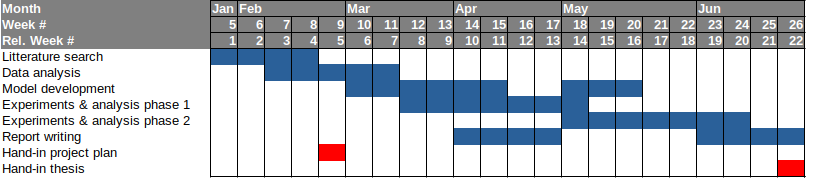
\includegraphics[width=0.8\textwidth]{time_plan.png}
\caption{Example Gantt chart of the project plan.}
\end{figure}

\newpage

\nocite{*}
\bibliographystyle{plain}
\bibliography{bibliography}

\end{document}
